\section{Logging throughput}
The 1000 user workload was the first occasion for our system to operate at nominal TPS for a significant portion of its runtime\improvement{link to image with 100 v 1000 tps}.
Since each transaction needed to write at least one entry to the audit log the volume of log messages was unprecedented.
Controlling the ``firehose'' of log messages was the most significant architectural redesign.
It included several false starts and, ultimately, reached a workable but flawed solution.

\subsection{Limits of logging to a flat file}
From the initial prototype through the 100 user workload, the audit service wrote directly to an \texttt{.xml} file that could be submitted for validation.
Log messages were removed from RMQ and stored in memory for writing by separate threads.
However, running the 1000 user workload exceeded the rate that the audit service could clear messages from RMQ, causing a significant backlog of messages to develop.
As the total message backlog size approached 700k the rate that messages could be exchanged slowed, causing a slowdown in the rest of the system as execution was blocked on message exchange.
Soon after, services would fail as they lost their connection to the RMQ server.

As noted in the ``Production Checklist'' section of the RMQ user guide\footnote{\url{https://www.rabbitmq.com/production-checklist.html}}, performance is heavily tied to available RAM.
As the backlog increases RMQ will begin swapping RAM to disk to ensure persistence.
The IO penalty for writing to disk causes an intense slowdown.
Since the worker services generating the logs are not capable of throttling they eventually push RMQ into resource exhaustion and failure.

Direct to file logging was never intended for production use.
Creating per-user dumplogs would be onerous since there was no direct method for searching or sorting the log file.
Leaving the log file implementation in place for most of the project allowed us to focus development efforts on optimizing the quote manager and implementing the auto transaction service.
Letting RMQ fail illuminated the ``danger zone'' for RMQ on the lab machines.
Different audit logger refactors could be compared for effectiveness by monitoring the RMQ backlog.

\subsection{Logging directly to an RDBMS}\label{sec:log-rdbms}
The first refactor involved inserting logs into Postgres and writing to a file on an as-requested basis.
This solved the problem of creating per-user log files but throughput was significantly worse than writing direct to a file.
With direct to file, the 100 user workload with 100k transactions generated 2k backlogged messages on RMQ.
With the Postgres refactor, the 100 user workload resulted in a 20k message backlog.
No attempts at larger workloads were made after this poor result.

This performance slowdown is not surprising.
The flat file and RDBMS both store the pre-formatted \texttt{.xml} entry for the event.
In addition, the RDBMS stores extra data about the user name, transaction type and creation time to enable queries.
The RDBMS is storing more data than the flat file.
In addition, the RDBMS suffers a performance penalty from indexing data on insertion.
While there are methods to mitigate these problems, such as connection pooling, the performance degredation was extreme enough to justify larger service refactors.

\subsection{Processing logs with ELK}
An RDBMS enables rich querying and enforces data integrity \textemdash{} useful features that are not relevant for storing an append-only log.
Moreover, the indexing that provides those useful features introduces a performance penalty that limits throughput.
Specialized log storage solutions forgo rich indexing in order to maximize write throughput.

The Elasticsearch - Logstash - Kibana (ELK) suite of applications from elastic.co\footnote{\url{https://www.elastic.co}} is a popular distributed log storage method.
Logstash consumes and transforms data for indexing and storage in Elasticsearch.
Kibana is a graphical monitoring suite that provides information about the logging rate and health of the logstash and elasticsearch services.

A prototype was created that deployed the ELK stack in separate Docker containers collocated with the audit logger.
Logstash consumed messages directly from RMQ and sent them to Elasticsearch for indexing and storage.
The prototype had abysmal performance.
With the 45 user workload there was a 7k (out of 10k total) backlog.
Development was abandoned at this point.

The poor performance of the ELK stack was directly related to its resource limitations.
Each part of the ELK stack performs better with more available RAM.
Collocating all services severely limited the available RAM.
Also, ELK requires a non-trivial amount of JVM and OS tuning to provide optimal resource availability.
Although there are guides for this process it was unclear how to apply their recommendations on the tower of abstractions in the production environment: a docker OS on a VM OS on a host OS, each needing their own tuning.

The Elasticsearch scaling guide\footnote{\url{https://www.elastic.co/guide/en/elasticsearch/guide/current/scale.html}} recommends adding more shards (i.e. independent instances which maintain a partition of the data) to increase write throughput.
This throughput solution \textemdash{} a distributed system within a distributed system \textemdash{} directly links scaling to resource demand.
Scaling Elasticsearch would likely reduce the number of systems available to host workers and limit the maximum TPS.
The problem of high log throughput would be solved by removing the ability to create logs at a high rate.

\subsection{Buffered logging}\label{sec:log-buf}
The problem with the RDBMS solution in~\ref{sec:log-rdbms} is fundamentally a mismatch between the production and consumption rate of log messages.
The solution to this problem is to place a buffer between the producer and consumer.

\begin{figure}[tbph]
  \centering
  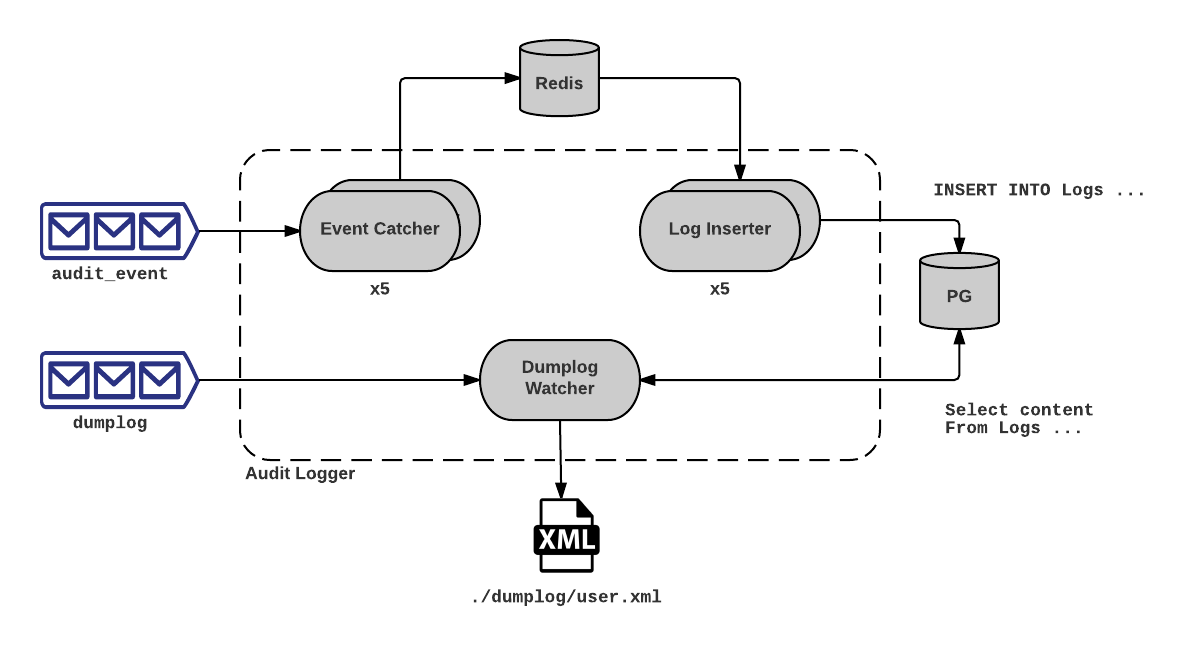
\includegraphics[width=0.95\linewidth]{graphics/audit}
  \caption{Buffered audit logger}
  \label{fig:audit}
\end{figure}

Figure~\ref{fig:audit} shows how multiple \texttt{Event Catcher} workers remove incoming log messages from RMQ and place them in Redis. \texttt{Log Inserter} workers remove items from Redis and store them in Postgres.
With this design, the 1000 user workload only reached a 20k backlog of messages and had no observed performance degradation.
Although a run would finish in around \SI{45}{\second} it would be upwards of \SI{6}{\minute} to finish insertion into Postgres.
When a message for a dumplog was processed it would display messages had successfully migrated to Postgres but was unaware of those still in Redis.
This is a soft violation of the business requirement that a dumplog should show all transactions proceeding itself.
We believe this is acceptable since, in actual use, there is no clear ``end of work'' to capture.
All log messages will make it into Postgres for querying so the requirement is \textit{eventually} satisfied.

This method has an upper limit to its effectiveness since the Redis buffer could run out of storage space under periods of sustained high TPS.
The boundary of the buffer memory was not encountered during any testing and we cannot speculate about its value.
In order to determine the limits we would need a workload file larger than the final workload.
Alternatively, we could induce a period of sustained high TPS by removing the requirement to re-fetch expired quotes and concatenate existing workloads.

\subsection{Alternate solutions}
When the buffer method in~\ref{sec:log-buf} reaches its limit there are several possible development paths for proceeding forward:

\begin{enumerate}
  \item \textit{Agglomerate messages}: Message traffic can be reduced by combining multiple log events into one message.
Workers would only emit messages for logging at fixed intervals or after a certain number of events (whichever comes first) and reduce the overhead associated with creating, sending and processing RMQ messages.
The optimal message size would have to be determined through experiment.
  \item \textit{RMQ scaling}: RMQ is capable of its own distributed deployment.
Increasing resources available to the message bus would allow more messages to be stored before removal into the buffer.
  \item \textit{Robust message passing}: Apache's Kafka\footnote{\url{https://kafka.apache.org}} provides functionality similar to RMQ but is optimized for message storage and large backlogs.
This allows consumers to operate at different rates and removes the need to process log messages faster.
\end{enumerate}
